\section{Initial dummy experimentation}
Before designing what would be the final orchestration scenario where everything would be synchronized and coordinated, I wanted to start from the very basics, the modular components. Before integrating the vision language model into the simulator framework, I preferred to experiment with the code available in the documentation. In order to gain an insight on how a VLM works from scratch, I did several experimentation \textit{notebooks} to practice with the basics.

\subsection{CLIP Demo Analysis}
The first modular practice I performed was experimenting with the \textit{CLIP} library and code available at the official GitHub repository \cite{openai_clip_2021}. I made a simple classification task notebook where the contrastive properties of CLIP would really shine. Consisting of a classification of an image among a set of custom labels and secondly a \textit{zero-shot classification} to check the zero-shot capabilities of the model. All of this code is available at path \texttt{/Scripts/Demos/} inside the project directory.

\subsubsection{Simple Classification}
Using the \textit{ViT-B/32} model CLIP offers inside its library, being a vision transformer for image classification, I have wanted the model to classify an image among a set of custom labels that image may belong to. As referenced in image \ref{fig:surfer_image}, the image to classify is a portray of a surfer riding a wave. The model must use its contrastive learning techniques it was trained with, and distinguish the image from a possible set of candidates being: a surfer (correct answer), a truck (incorrect) and a mountain (incorrect).

\begin{figure}[H]
	\centering 
	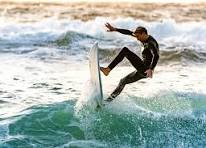
\includegraphics[width=.3\textwidth]{imgs/surfer.png}
	\label{fig:surfer_image}
	\caption{Image to classify used in the CLIP features demonstration notebook, showing a surfer.}
\end{figure}

After processing and encoding the features of the image and \textit{tokenizing} the labels of the candidates, calculates the probabilities of the image belonging to each label. Returning a probability distribution that sums up to 1 because of the \textit{softmax} activation function. Looking at the results, the vision transformer trained with CLIP's contrastive learning approach had no problem identifying the winner. Reflecting CLIP's astonishing performance for simple classification tasks, however, the second sub-task is a little bit more difficult.

\begin{quote}
	\textbf{Label probabilities}: [[9.9999571e-01 2.2835159e-06 2.0020473e-06]]
\end{quote}

\subsubsection{Zero-Shot Classification with CLIP}
Loading the \textit{CIFAR100} well-known dataset for including thousands of colored images belonging to 100 different classes, the same vision-transformer must generate text descriptions for all of the 100 classes of the dataset and taking a random sample instance calculate the similarity between the image's visual inputs and each of the generated descriptions. Basically a zero-shot classification task, where the model must predict the answer without any previous knowledge, just based on the generated text captions.

\begin{quote}
	\textbf{Selected image:} \texttt{snake image} \\
	\textbf{Top 5 predictions:} \\
	\texttt{snake: 65.31\% \\ turtle: 12.29\% \\ sweet\_pepper: 3.83\% \\ lizard: 1.88\% \\ crocodile: 1.75\%}
\end{quote}

Great results  as the model gets the correct answer sharing a pretty well distributed probability. As while getting the best result the next most probable ones are all green animals or green food, showing great zero-shot classification performance.

\subsubsection{Image Captioning with BLIP}
I also tried other tasks as image captioning with other VLM models such as BLIP. Having the same surfer image \ref{fig:surfer_image} as input, the model did describe it surprisingly well for a maximum number of tokens like 30. Being its short description for the image: 

\begin{quote}
	\textbf{Caption:} \textit{a man riding a wave on top of a surfboard}
\end{quote}

\subsubsection{Visual Question Answering}
Question answering also returned great results. Still using BLIP and the same surfer photo, I asked the model a rather complicated question. 

\begin{quote}
	\textbf{Question}: \textit{What color is the surfer's board?} \textbf{Answer}: \textit{white}
\end{quote}

The question of what is the color of the surfboard seems easier than what it actually is, as the model must be able to distinguish between the board and the white foam parts of the waves. Which is already struggling to the human eye. Even if the question was tricky reason why I chose both the question and this image, the model got it correct once again. 

\section{IsaacSim environment design}
agents, cameras, physics, ...

\subsection{First scenarios}

\subsection{Last scenario}

\section{VLM integration}
Mention the already implemented VLM part in IsaacSim

\section{Agent Control}

\section{Communication layer} % ?